\documentclass[11pt]{article}
\usepackage{amsmath,amssymb,amsthm}
\usepackage[margin=1in]{geometry}
\usepackage{array}
\usepackage{tabularx}
\usepackage{booktabs}
\usepackage{tikz}
\usepackage{float}
\usepackage[hidelinks]{hyperref}

\theoremstyle{plain}
\newtheorem{theorem}{Theorem}[section]
\newtheorem{lemma}[theorem]{Lemma}
\newtheorem{proposition}[theorem]{Proposition}
\newtheorem{corollary}[theorem]{Corollary}
\theoremstyle{definition}
\newtheorem{definition}[theorem]{Definition}
\newtheorem{example}[theorem]{Example}
\newtheorem{fact}[theorem]{Fact}
\newtheorem{observation}[theorem]{Observation}
\theoremstyle{remark}
\newtheorem{remark}[theorem]{Remark}

\newcommand{\Z}{\mathbb{Z}}
\newcommand{\sm}{\setminus}
\DeclareMathOperator{\exc}{exc}
\newcommand{\dg}{\operatorname{deg}}

\title{Shortest-side skeletons of edge-perimeter-minimizing polyhexes}
\author{H. Utsunomiya}
\date{}

\begin{document}
\maketitle

\begin{abstract}
A polyhex is a finite connected set of cells of the hexagonal tiling, and its edge perimeter
is the number of unit edges separating it from its complement. The minimum edge perimeter
for a given number of cells is classical, and so is the existence of one nested sequence of
minimizers, one for each size. We prove a structural statement about \emph{all} minimizers:
deleting any shortest extreme line from a minimizer with at least three cells leaves a
minimizer whose minimum edge semiperimeter (the \emph{threshold} of its size) has dropped
by exactly one, and the deleted line can be restored
one cell at a time through configurations whose edge perimeter exceeds the minimum for
their size by at most two. Consequently every minimizer lies on a chain of minimizers linked
by such deletions, and every minimizer can be built from a single cell by adding one
adjacent cell at a time with edge-perimeter excess never above two. The constant two cannot
be lowered: the skeleton of minimizers exists for every minimizer, but not every minimizer
lies on a nested sequence of minimizers at the level of single cells. The proof rests on the
tight hull of a configuration, its exact defect identity, and a rigidity statement at the
plateau starts whose threshold is \(3\) or \(5\) modulo \(6\).
\end{abstract}

\noindent\textit{2020 Mathematics Subject Classification.} Primary 05B50; Secondary 05C35,
52C20.

\noindent\textit{Key words and phrases.} polyhex, edge-isoperimetric problem, minimum edge
perimeter, edge-perimeter minimizer, nested solutions, one-cell growth sequence, triangular
lattice, hexagonal tiling.

\section{Introduction}\label{sec:intro}

\subsection{The question}\label{sec:0.1}

Cells of the hexagonal tiling are the objects; a \emph{polyhex} is a finite connected set of
them, and its \emph{edge perimeter} \(p(S)\) is the number of unit edges with exactly one
side in \(S\). Writing \(p_{\min}(N)\) for the least edge perimeter of an \(N\)-cell
polyhex and
\[
   \exc(S):=p(S)-p_{\min}(|S|)
\]
for the \emph{excess}, a \emph{minimizer} is a polyhex with \(\exc=0\).

The static problem --- what is \(p_{\min}(N)\), and what do minimizers look like --- is
classical. The question here is dynamic. A minimizer is a finished object; can it be
\emph{assembled}, one cell at a time, without ever leaving the neighbourhood of optimality?
Formally, given an \(N\)-cell minimizer \(S\), is there a chain
\[
   S_{1}\subset S_{2}\subset\cdots\subset S_{N}=S,\qquad |S_{k}|=k,
\]
of polyhexes in which each step adds a single adjacent cell and every \(S_{k}\) has small
excess?

Two remarks fix the difficulty. First, one cannot ask for \(\exc(S_{k})=0\) throughout: we
exhibit a \(13\)-cell minimizer from which no single cell can be removed to leave a
\(12\)-cell minimizer. Second, the natural greedy reading of the question is false: it is
not true that every configuration of excess at most two admits a one-cell deletion keeping
the excess at most two, and a \(31\)-cell directionally convex example in
Remark~\ref{rem:x31} has no such downward move. Thus the entire class \(\{\exc\le2\}\)
cannot serve as the state space of a one-cell downward induction with a universally
available move.

\subsection{Results}\label{sec:0.2}

The answer is that the growth has a \emph{skeleton} made of minimizers. For a polyhex \(S\),
the six \emph{extreme lines} are the outermost occupied lines in the three lattice
directions, and a \emph{shortest} extreme line is one carrying the fewest cells of \(S\).
For a minimizer the cells of \(S\) on each extreme line form a contiguous run; that is a
theorem (Theorem~\ref{thm:capacity}(d)), and Definition~\ref{def:traces} states the notion
on the class of polyhexes for which it holds. Write \(g(N):=\lceil\sqrt{12N-3}\,\rceil\),
so that \(p_{\min}(N)=2g(N)\) by a classical result recalled in
Section~\ref{sec:capacity}. We call \(g(N)\) the \emph{threshold} of \(N\): it is the
least edge semiperimeter an \(N\)-cell polyhex can have, and it is constant on runs of
consecutive \(N\) that we call \emph{plateaus}. The excess of a polyhex \(S\) is
\[
   \exc(S)=p(S)-p_{\min}(|S|)=2\bigl(\sigma(S)-g(|S|)\bigr),
\]
where \(\sigma(S)=p(S)/2\) is its edge semiperimeter.

\begin{theorem}[shortest-side skeleton]\label{thm:intro-skel}
Let \(S\) be an edge-perimeter minimizer with \(|S|\ge3\) and let \(\Lambda\) be any
shortest extreme line of \(S\). Then \(S\sm\Lambda\) is an edge-perimeter minimizer with
\(g(|S\sm\Lambda|)=g(|S|)-1\), and the cells of \(S\cap\Lambda\) can be restored one at a
time through polyhexes of excess at most two.
\end{theorem}

Iterating, every minimizer \(S\) admits a chain
\(S=T_{0}\supset T_{1}\supset\cdots\supset T_{k}\) of minimizers, \(|T_{k}|\le2\), each
obtained from the previous one by deleting a shortest extreme line. Interpolating each
step and reading the result backwards gives the growth statement.

\begin{theorem}[one-cell growth]\label{thm:intro-main}
Let \(S\) be an \(N\)-cell polyhex of minimum edge perimeter. Then there are polyhexes
\(S_{1}\subset\cdots\subset S_{N}=S\) with \(|S_{k}|=k\) such that
\begin{enumerate}
\item[(a)] for each \(k<N\), the polyhex \(S_{k+1}\) is obtained from \(S_{k}\) by adding one
cell adjacent to \(S_{k}\), and
\item[(b)] \(\exc(S_{k})\le2\) for every \(k\).
\end{enumerate}
\end{theorem}

Equivalently, writing \(\mathcal{M}_{N}\) for the \(N\)-cell minimizers and
\(\mathcal{R}_{N}\) for the \(N\)-cell polyhexes reachable from a single cell by one-cell
growth with excess never above two, \(\mathcal{M}_{N}\subseteq\mathcal{R}_{N}\): restricting
candidate generation to such growth excludes no minimizer.

\begin{theorem}[optimality of the constant]\label{thm:intro-sharp}
The constant two in Theorem~\ref{thm:intro-main} cannot be lowered.
\end{theorem}

Since \(p\) and \(p_{\min}\) are both even, the excess is always an even non-negative
integer, so the only smaller uniform bound would be zero; the \(13\)-cell configuration
mentioned above rules that out. Theorems~\ref{thm:intro-skel} and~\ref{thm:intro-sharp}
together locate the cost precisely: the skeleton of minimizers can always be kept optimal,
and the excess \(2\) is spent only while a single extreme line is being rebuilt cell by cell.

\subsection{How the proof works}\label{sec:0.3}

Three ingredients carry the argument. First, every minimizer is \emph{directionally
convex}: along each of the three lattice directions its trace on every line is a single
run. This follows from a comparison with the \emph{tight hull} of the configuration, the
lattice hexagon spanned by its extreme lines, whose cell count satisfies an exact
\emph{defect identity} in terms of its six side lengths. The same identity yields the
capacity function \(M(t)=\lfloor(t^{2}+3)/12\rfloor\), the largest number of cells that fit
within an edge-semiperimeter budget of \(t\), and with it the formula for \(p_{\min}\).

Second, the six side lengths of the hull add up to exactly three more than the number of
occupied lines, so a shortest extreme line of a minimizer with threshold \(\sigma\) carries at
most \(\lfloor(\sigma+3)/6\rfloor\) cells. A residue computation modulo \(6\) shows that
deleting that many cells from a minimizer lands on a minimizer one threshold step down ---
except possibly when the threshold is \(3\) or \(5\) modulo \(6\), the minimizer sits at the
very start of its plateau, and the shortest line is as long as the bound allows.

Third, if in that exceptional situation the shortest trace attained the bound, the hull
would be forced to be a regular hexagon, or a regular hexagon with one pair of opposite
sides lengthened by one, and its boundary would then force the minimizer to fill the hull
completely; but the plateau start has strictly fewer cells than that hexagon. This
\emph{rigidity} closes the last case. Restoring the deleted line one cell at a
time never raises the perimeter above its starting value, while the threshold has already
dropped by one, which is where the excess \(2\) comes from.

\subsection{The role of computation}\label{sec:0.4}

No theorem in this paper depends on finite enumeration, and neither does
Theorem~\ref{thm:intro-sharp}. Computation appears in Section~\ref{sec:computation} for
two purposes: to determine, by complete enumeration, that \(13\) is the smallest size at
which a minimizer has no all-minimizer growth chain --- a question the analytic arguments
do not answer; and to re-check the statements of the paper at small sizes with
implementations independent of their proofs.

\subsection{Relation to previous work}\label{sec:0.5}

The cell-adjacency graph of the hexagonal tiling is the triangular lattice
with its unit-distance edges, and the edge boundary of a set of cells in that
graph is exactly its edge perimeter; the problem studied here is therefore the
edge-isoperimetric problem on the triangular lattice. Its minimum value
$p_{\min}(N)=2\lceil\sqrt{12N-3}\,\rceil$ is due to Harary and Harborth
\cite{HararyHarborth1976}.
Since an $N$-cell polyhex with $b$ adjacent pairs has edge perimeter $6N-2b$,
this value corresponds to Harborth's earlier formula
$\lfloor 3N-\sqrt{12N-3}\rfloor$ for the maximum number of touching pairs among
$N$ non-overlapping unit discs in the plane \cite{Harborth1974}. The capacity function $M(t)$
coincides, when their perimeter variable is set equal to $t+3$, with the
maximum-size function of F\"ulep and Sieben for the site perimeter of polyhexes
\cite[Proposition~5.10]{FulepSieben2010}, for every $t\ge 3$ other than $t=4$
(Remark~\ref{rem:fs}); and
our hull defect identity corresponds to their polyiamond identity
\cite[Lemma~3.3]{FulepSieben2010} under the duality of their Section~5. The two perimeters are
different functionals (Remark~\ref{rem:site}); only the resulting formulas correspond.
Section~\ref{sec:capacity} rederives these facts in edge-perimeter variables because the proof
needs the hull machinery, not merely the values.

Davoli, Piovano and Stefanelli \cite{DavoliPiovanoStefanelli2017} study the same
edge-isoperimetric problem and characterize all minimizers. They prove, in particular,
that minimizers are directionally convex (see the remark after
Theorem~\ref{thm:capacity}). Their results do not state that deleting a shortest
extreme line preserves minimality, nor the bounded-excess one-cell growth statement
proved here.

The triangular-lattice edge-isoperimetric problem admits a nested solution
\cite[Theorem~7.2, p.~135]{Harper2004}: an ordering of the lattice whose every finite
prefix is optimal. Vainsencher and Bruckstein \cite{VainsencherBruckstein2008}
observe that a spiral construction attains the optimal perimeter at every size
without exhausting the optimal shapes. Malen, Rold\'an and Toal\'a-Enr\'iquez
\cite{MalenRoldanToala2023} extend the spiral construction to Euclidean and
hyperbolic $\{p,q\}$-animals. A nested solution supplies one minimizer at each
size; the present results concern every prescribed minimizer.
Theorem~\ref{thm:intro-skel} gives a chain of minimizers through each of them when
steps delete whole extreme lines, whereas Theorems~\ref{thm:intro-main}
and~\ref{thm:intro-sharp} show that an excess of two is sufficient and necessary
for one-cell growth to reach all minimizers.

\subsection{Organization}\label{sec:0.6}

Of the results below, the minimum edge perimeter and the capacity function
(Section~\ref{sec:capacity}), the tight-hull identities (Section~\ref{sec:hulls}) and the directional
convexity of minimizers (Theorem~\ref{thm:capacity}(d)) are classical or close to known
results, as explained in Section~\ref{sec:0.5}, and are proved here only to keep the
argument self-contained in the variables it needs. The contribution of the
paper is Theorems~\ref{thm:intro-skel}--\ref{thm:intro-sharp}.

Sections~\ref{sec:prelim}--\ref{sec:capacity} fix the lattice, the edge perimeter,
directional convexity, the tight hull and its identities, and the capacity function.
Section~\ref{sec:rigidity} bounds the shortest extreme line and proves the rigidity
statement at exceptional plateau starts. Section~\ref{sec:skeleton} proves the skeleton
theorem and derives Theorem~\ref{thm:intro-main}. Section~\ref{sec:sharp} proves that the
constant two is optimal. Section~\ref{sec:remarks} records what the argument does not
give, and Section~\ref{sec:computation} the computational checks.


\section{The hexagonal lattice, runs, and directional convexity}\label{sec:prelim}

Sections~\ref{sec:prelim}--\ref{sec:capacity} fix the lattice, the perimeter functional,
the convexity notion, the tight hull and its identities, and the extremal capacity function.
The proof of the main theorem in Sections~\ref{sec:rigidity}--\ref{sec:skeleton} reads all
of its geometry from here.

\subsection{Lattice and polyhexes}\label{sec:2.1}

Cells of the hexagonal tiling are indexed by axial coordinates
\((q,r)\in\Z^{2}\). We call \(q\), \(r\) and
\[
   s:=q+r
\]
the three \emph{keys} of a cell; in words, the third key of a cell is the sum of its two
axial coordinates. Two cells are \emph{adjacent} when they differ by one of the six
vectors
\[
   d_{0}=(1,0),\quad d_{1}=(0,1),\quad d_{2}=(-1,1),\quad
   d_{3}=(-1,0),\quad d_{4}=(0,-1),\quad d_{5}=(1,-1).
\]

A \emph{polyhex} is a finite nonempty set of cells that is connected with respect to
adjacency. We write \(|S|\) for the number of cells of \(S\).

The following four facts are immediate from the definitions and are used throughout
without further comment.

\begin{fact}\label{f:1}
Two distinct cells are adjacent if and only if they agree in exactly one key and differ
by exactly \(1\) in the other two. In words: an adjacency step keeps one of the three
keys fixed and changes each of the other two by one unit (the step \(d_{0}=(1,0)\), for
instance, sends \((q,r,s)\) to \((q+1,r,s+1)\), so the two changing keys need not move
in opposite senses).
\end{fact}

\begin{proof}
Each \(d_{j}\) changes \((q,r,s)\) by \((1,0,1)\), \((0,1,1)\), \((-1,1,0)\),
\((-1,0,-1)\), \((0,-1,-1)\) or \((1,-1,0)\). There are twelve triples
\((\Delta q,\Delta r,\Delta s)\) with one zero entry and two entries equal to
\(\pm1\); exactly six of them satisfy \(\Delta s=\Delta q+\Delta r\), and they are
the six just listed. Conversely a difference of that shape is one of the \(d_{j}\).
\end{proof}

\begin{fact}\label{f:2}
A \emph{line} is a set of cells on which one key is constant. Two lines belonging to
different keys meet in exactly one cell; two distinct lines belonging to the same key are
disjoint.
\end{fact}

\begin{fact}\label{f:3}
One adjacency step changes each of \(q\), \(r\) and \(s\) by at most \(1\).
\end{fact}

\begin{fact}\label{f:4}
For a polyhex \(S\) and each key, the set of values taken by that key on \(S\) is an
interval of consecutive integers. In words: no key value inside the range of \(S\) can be
skipped.
\end{fact}

\begin{proof}
Let \(k\) be a key and let \(x,y\in S\) realize two values of \(k\). A path of adjacent
cells inside \(S\) joins them, and by Fact~\ref{f:3} the value of \(k\) changes by at most
one per step, so every intermediate integer occurs on the path.
\end{proof}

\subsection{Edge perimeter, runs and directional convexity}\label{sec:2.2}

Let \(a(S)\) denote the number of unordered pairs of adjacent cells of \(S\). The
\emph{edge perimeter} of \(S\) is
\begin{equation}\label{eq:p}
   p(S)=6|S|-2a(S),
\end{equation}
in words: six times the number of cells, minus twice the number of adjacent pairs.
Equivalently, \(p(S)\) counts the cell edges of \(S\) that are not shared with another
cell of \(S\); we call these the \emph{boundary edges}. The \emph{edge semiperimeter} is
\[
   \sigma(K):=\tfrac{1}{2}p(K)
\]
for any finite set of cells \(K\); in words, half the edge perimeter. That this is an
integer is part of Lemma~\ref{lem:runs} below.

A line \(\Lambda\) is \emph{occupied} by \(S\) when \(S\cap\Lambda\neq\emptyset\); we call
\(S\cap\Lambda\) the \emph{trace} of \(S\) on \(\Lambda\). Cells of a line are linearly
ordered (for a line of constant \(q\) by the value of \(r\), for one of constant \(r\) by
the value of \(q\), for one of constant \(s\) by the value of \(q\)), and consecutive
cells in that order are adjacent. A \emph{run} of \(S\) on \(\Lambda\) is a maximal block
of consecutive cells of the trace. Let
\[
   R(S)=\text{the total number of runs of \(S\) over all lines},\qquad
   \lambda(S)=\text{the number of occupied lines}.
\]

\begin{definition}\label{def:dconv}
A polyhex \(S\) is \emph{directionally convex} when the trace of \(S\) on every occupied
line is a single run. In words: along each of the three directions, \(S\) never leaves a
line and comes back to it.
\end{definition}

This is a lattice notion and not Euclidean convexity; it is the notion called
\emph{layer convexity} in parts of the literature on lattice animals.

\begin{lemma}\label{lem:runs}
For every finite set of cells \(S\),
\begin{equation}\label{eq:pruns}
   p(S)=2R(S)\ \ge\ 2\lambda(S),
\end{equation}
in words: the edge perimeter equals twice the total number of runs, and the total number
of runs is at least the number of occupied lines. In particular \(p(S)\) is even and
\(\sigma(S)=R(S)\). For a polyhex, equality \(R(S)=\lambda(S)\) holds if and only if
\(S\) is directionally convex.
\end{lemma}

\begin{proof}
Let \(e=\{x,y\}\) be a boundary edge, with \(x\in S\) and \(y\notin S\) the two cells it
separates. By Fact~\ref{f:1} the cells \(x\) and \(y\) agree in exactly one key, hence
they are consecutive cells of exactly one line \(\Lambda\), and \(x\) is an end of the run
of \(S\) on \(\Lambda\) containing it. Conversely a run has exactly two ends, and the cell
immediately beyond each end lies outside \(S\) and determines a boundary edge; for a run
consisting of a single cell the two ends are the two opposite sides of that cell, so they
give two distinct boundary edges. This is a bijection between boundary edges and ends of
runs, whence \(p(S)=2R(S)\).

Every occupied line carries at least one run, so \(R(S)\ge\lambda(S)\), with equality
exactly when every occupied line carries exactly one run, which is
Definition~\ref{def:dconv}.
\end{proof}

\begin{remark}[edge perimeter versus site perimeter]\label{rem:site}
The \emph{site perimeter} of $S$ is the number of cells outside $S$ adjacent to at
least one cell of $S$. It is a different functional from \eqref{eq:p}, and the two have
different minimizers in general; results about one do not transfer to the other.
F\"ulep and Sieben \cite{FulepSieben2010} use the site perimeter. The correspondence
with their formulas described in Section~\ref{sec:0.5} and Remark~\ref{rem:fs} is
algebraic; the proofs here use the edge perimeter throughout.
\end{remark}

\subsection{Extreme support lines and traces}\label{sec:2.3}

Let \(S\) be a polyhex. For each key, Fact~\ref{f:4} makes the occupied values an interval,
so there is a smallest and a largest occupied line in each of the three families. These six
lines are the \emph{extreme lines} of \(S\); we list them in the cyclic order
\[
   \Lambda_{1}:\ q=q_{\min},\quad
   \Lambda_{2}:\ r=r_{\max},\quad
   \Lambda_{3}:\ s=s_{\max},\quad
   \Lambda_{4}:\ q=q_{\max},\quad
   \Lambda_{5}:\ r=r_{\min},\quad
   \Lambda_{6}:\ s=s_{\min},
\]
so that \(\Lambda_{i}\) and \(\Lambda_{i+3}\) are the two extreme lines of one and the same
family, indices being read in \(\Z/6\). If a family occupies a single line then the two
corresponding extreme lines coincide; all statements below are read with that degeneracy
allowed.

\begin{definition}\label{def:traces}
Let \(S\) be a \emph{directionally convex} polyhex. Its six \emph{support traces} are the
traces \(S\cap\Lambda_{i}\), each a single run by Definition~\ref{def:dconv}, and we write
\[
   r_{i}:=|S\cap\Lambda_{i}|\ \ge 1 ,\qquad i\in\Z/6,
   \qquad\text{and}\qquad
   \rho(S):=\min_{i} r_{i} .
\]
\end{definition}

The six extreme lines of \(S\) will turn out to be the six side lines of its tight hull
(Lemma~\ref{lem:hull}(ii)); from then on the same symbol \(\Lambda_i\) serves both
roles, and the start of Section~\ref{sec:rigidity} fixes the terminology for the two
finite sets, side and support trace, that live on it.

\begin{remark}\label{rem:rho}
Definition~\ref{def:traces} is stated for directionally convex \(S\) only. On that domain \(\rho(S)\) is at once the length of the shortest support trace and the
length of the shortest extreme-line run. For
a general polyhex a trace need not be a run, and we do not extend the definition.
\end{remark}


\section{Tight hulls and exact identities}\label{sec:hulls}

\subsection{Tight lattice hulls}\label{sec:2.4}

\begin{definition}\label{def:hexagon}
Let \(L\ge1\) and \(u,v,w\ge0\) be integers satisfying the \emph{admissibility} conditions
\begin{equation}\label{eq:adm}
   u+v\le L-1,\qquad v+w\le L-1,\qquad u+w\le L-1 ,
\end{equation}
and put \(A:=L-u\), \(B:=L-v\), \(C:=L-w\), so that \(A,B,C\ge1\). The corresponding
\emph{lattice hexagon} is
\[
   H(L;u,v,w):=\{\,(q,r):\ 0\le q\le A-1,\ \ 0\le r\le B-1,\ \ w\le q+r\le L-1\,\}.
\]
In words: the triangle of side \(L\) with three corner triangles of sides \(u\), \(v\) and
\(w\) cut off. Degenerate shapes, in which one or more of the cut corners is empty or one
of the three widths equals \(1\), are allowed.
\end{definition}

\begin{definition}\label{def:hull}
The \emph{tight hull} \(H(S)\) of a polyhex \(S\) is the lattice hexagon determined by the
extreme values of the three keys on \(S\). Concretely, normalize by a translation so that
\(q_{\min}=r_{\min}=0\) and set
\[
   A=1+q_{\max},\quad B=1+r_{\max},\quad L=1+s_{\max},\quad w=s_{\min},\quad
   u=L-A,\quad v=L-B .
\]
\end{definition}

For this to define a lattice hexagon in the sense of Definition~\ref{def:hexagon}, the
four parameters must be admissible. They are.

\begin{lemma}[the tight hull is admissible]\label{lem:tightadm}
For every polyhex \(S\), the parameters \(L,u,v,w\) of Definition~\ref{def:hull} satisfy
\(L\ge1\), \(u,v,w\ge0\) and the three inequalities \eqref{eq:adm}. Hence
\(H(S)=H(L;u,v,w)\) is a lattice hexagon.
\end{lemma}

\begin{proof}
After the normalization \(q_{\min}=r_{\min}=0\), every cell of \(S\) has \(q,r\ge0\),
hence \(s=q+r\ge0\); so \(w=s_{\min}\ge0\) and \(L=1+s_{\max}\ge1\). In the notation
of the definition, \(u=s_{\max}-q_{\max}\) and \(v=s_{\max}-r_{\max}\), and the four
remaining conditions are the following four inequalities between extreme values, each
read off from one well-chosen cell of \(S\).
\begin{itemize}
\item \(u\ge0\) and \(v\ge0\): a cell with \(q=q_{\max}\) has \(s=q_{\max}+r\ge q_{\max}\),
so \(s_{\max}\ge q_{\max}\); likewise \(s_{\max}\ge r_{\max}\).
\item \(u+v\le L-1\), that is \(s_{\max}\le q_{\max}+r_{\max}\): a cell with
\(s=s_{\max}\) has \(s_{\max}=q+r\le q_{\max}+r_{\max}\).
\item \(v+w\le L-1\), that is \(s_{\min}\le r_{\max}\): a cell with \(q=q_{\min}=0\) has
\(s=r\le r_{\max}\), so \(s_{\min}\le r_{\max}\).
\item \(u+w\le L-1\), that is \(s_{\min}\le q_{\max}\): a cell with \(r=r_{\min}=0\) has
\(s=q\le q_{\max}\).
\end{itemize}
Note that only the six extreme values are used, not connectedness.
\end{proof}

For a lattice hexagon \(H\) we write \(\Lambda_{1},\dots,\Lambda_{6}\) for its six extreme
lines in the cyclic order of Section~\ref{sec:2.3}, namely
\[
   q=0,\quad r=B-1,\quad s=L-1,\quad q=A-1,\quad r=0,\quad s=w ,
\]
and call them the \emph{side lines}; we write
\[
   \ell_{i}:=|H\cap\Lambda_{i}|
\]
for the six \emph{side lengths}, \(h:=\min_{i}\ell_{i}\) for the shortest side length, and
\(\kappa_{i}:=H\cap\Lambda_{i}\cap\Lambda_{i+1}\) for the \emph{corner} cells. Finally we
set
\[
   \delta(H):=\ell_{1}-\ell_{4},
   \qquad
   Q(H):=(\ell_{1}-\ell_{3})^{2}+(\ell_{3}-\ell_{5})^{2}+(\ell_{5}-\ell_{1})^{2} .
\]

\begin{lemma}\label{lem:hull}
Let \(S\) be a polyhex and \(H=H(S)\). Then
\begin{enumerate}
\item[(i)] \(S\subseteq H\);
\item[(ii)] \(S\) and \(H\) occupy exactly the same lines, so \(\lambda(S)=\lambda(H)\);
\item[(iii)] each of the six side lines of \(H\) meets \(S\).
\end{enumerate}
\end{lemma}

\begin{proof}
(i) is immediate from Definition~\ref{def:hull} and Lemma~\ref{lem:tightadm}, since
every cell of \(S\) satisfies the six inequalities defining \(H\). For (ii), the lines occupied by \(S\) in the \(q\)-family
are, by Fact~\ref{f:4}, exactly \(q=0,\dots,A-1\), and likewise \(r=0,\dots,B-1\) and
\(s=w,\dots,L-1\); these are precisely the lines occupied by \(H\), as read off from
Definition~\ref{def:hexagon}. Assertion (iii) is the case of (ii) for the six extreme
values: each of them is attained by some cell of \(S\).
\end{proof}

Lemma~\ref{lem:hull} is the only place where connectedness of \(S\) is used in this
section, and it is used through Fact~\ref{f:4}: for a disconnected set the occupied key
values need not form an interval, and (ii) fails.

\subsection{Hull identities}\label{sec:2.5}

\begin{lemma}\label{lem:hex}
Let \(H=H(L;u,v,w)\) be a lattice hexagon. Then:
\begin{enumerate}
\item[(i)] the six side lengths are
\[
   \ell_{1}=L-v-w,\quad \ell_{2}=v+1,\quad \ell_{3}=L-u-v,\quad
   \ell_{4}=u+1,\quad \ell_{5}=L-u-w,\quad \ell_{6}=w+1 ,
\]
and each side line meets \(H\) in a single run whose two end cells are the corners
\(\kappa_{i-1}\) and \(\kappa_{i}\);
\item[(ii)] \(H\) is a directionally convex polyhex with
\[
   \lambda(H)=\sigma(H)=A+B+C=3L-(u+v+w);
\]
\item[(iii)] the six side lengths satisfy
\begin{equation}\label{eq:sidesum}
   \sum_{i=1}^{6}\ell_{i}=\lambda(H)+3 ,
\end{equation}
in words: the six side lengths of the hull add up to three more than the number of lines
the hull occupies; and the three differences across opposite sides agree,
\begin{equation}\label{eq:delta}
   \ell_{1}-\ell_{4}=\ell_{3}-\ell_{6}=\ell_{5}-\ell_{2}=\delta(H)=L-u-v-w-1 ;
\end{equation}
\item[(iv)] with \(T(k):=k(k+1)/2\),
\[
   |H|=T(L)-T(u)-T(v)-T(w) ;
\]
\item[(v)] \textup{(hull defect identity)}
\begin{equation}\label{eq:defectid}
   \lambda(H)^{2}+3-12|H| \;=\; 3\,\delta(H)^{2}+2\,Q(H)\;\ge\;0 ,
\end{equation}
in words: the square of the number of occupied lines, plus three, minus twelve times the
number of cells, equals three times the square of the common opposite-side difference plus
twice the imbalance \(Q(H)\).
\end{enumerate}
\end{lemma}

\begin{proof}
(i) On the line \(q=0\) the defining inequalities reduce to \(w\le r\le\min(B-1,L-1)=B-1\),
which is a nonempty interval because \(w\le B-1\) is the condition \(v+w\le L-1\) of
\eqref{eq:adm}; its length is \(B-w=L-v-w\). On the line \(r=B-1\) they reduce to
\(\max(0,w-B+1)\le q\le\min(A-1,v)\), and \eqref{eq:adm} gives \(w-B+1\le0\) and
\(v\le A-1\), so the interval is \(0\le q\le v\), of length \(v+1\). The remaining four
sides are obtained in the same way, each time using exactly one of the three inequalities
of \eqref{eq:adm} at each end. Each side is an interval of consecutive cells of its line,
hence a run; its two end cells are the two cells where a second defining inequality becomes
an equality, that is, the two corners.

(ii) The occupied lines are \(q=0,\dots,A-1\), \(r=0,\dots,B-1\) and \(s=w,\dots,L-1\),
which number \(A+B+C\); on each of them the trace is an interval of consecutive cells by
the same computation as in (i), so \(H\) is directionally convex and
Lemma~\ref{lem:runs} gives \(\sigma(H)=R(H)=\lambda(H)\). Connectedness follows since each
trace is a run and consecutive traces meet a common line.

(iii) Summing the six expressions of (i),
\[
   \sum_{i}\ell_{i}=3L-(u+v+w)+3=\lambda(H)+3 .
\]
Using the side-length formulas of (i), the three opposite-side differences
\(\ell_{1}-\ell_{4}\), \(\ell_{3}-\ell_{6}\), \(\ell_{5}-\ell_{2}\) of \eqref{eq:delta}
are \((L-v-w)-(u+1)\), \((L-u-v)-(w+1)\) and \((L-u-w)-(v+1)\), all equal to
\(L-u-v-w-1\).

(iv) The triangle \(\{q,r\ge0,\ q+r\le L-1\}\) has \(T(L)\) cells. The three sets removed
in Definition~\ref{def:hexagon} are the corner triangles \(q\ge A\), \(r\ge B\) and
\(q+r\le w-1\), of \(T(u)\), \(T(v)\) and \(T(w)\) cells respectively, and \eqref{eq:adm}
makes them pairwise disjoint: a cell with \(q\ge A\) and \(r\ge B\) would have
\(q+r\ge A+B=2L-u-v\ge L+1\), which is impossible, and a cell with \(q\ge A\) and
\(q+r\le w-1\) would give \(r\le w-1-A<0\), and symmetrically.

(v) Put \(U:=u+v+w\) and \(P:=u^{2}+v^{2}+w^{2}\). By (ii) and (iv),
\[
   \lambda(H)^{2}+3-12|H|=(3L-U)^{2}+3-6L(L+1)+6P+6U
   =3L^{2}-6LU-6L+U^{2}+6P+6U+3 .
\]
On the other side, \(\delta(H)=L-U-1\) and, by (i),
\(Q(H)=(u-w)^{2}+(w-v)^{2}+(v-u)^{2}=3P-U^{2}\), so
\[
   3\delta(H)^{2}+2Q(H)=3(L-U-1)^{2}+2(3P-U^{2})
\]
expands to the same expression. In words: both sides equal three times \(L^{2}\), minus six
times \(LU\), minus six times \(L\), plus \(U^{2}\), plus six times \(P\), plus six times
\(U\), plus three. Nonnegativity is clear from the right-hand side.
\end{proof}


Write \(h:=\min_{i}\ell_{i}\) for the shortest side length and
\[
   x_{i}:=\ell_{i}-h\ \ge0
\]
for the \emph{side excess}, the amount by which a hull side exceeds the shortest one.

\begin{lemma}[opposite-side excess]\label{lem:oppair}
If \(\sum_{i}x_{i}\le2\) then \(x_{i}=x_{i+3}\) for every \(i\); in particular
\(\sum_{i}x_{i}\) is even, so \(\sum_{i}x_{i}=1\) is impossible, and if
\(\sum_{i}x_{i}=2\) then exactly one pair of opposite sides has length \(h+1\) and the other
four sides have length \(h\).
\end{lemma}

\begin{proof}
Since the \(x_{i}\) differ from the \(\ell_{i}\) by the constant \(h\), \eqref{eq:delta}
gives \(x_{1}-x_{4}=x_{3}-x_{6}=x_{5}-x_{2}=\delta(H)\). If \(\delta(H)\ge1\) then
\(x_{1},x_{3},x_{5}\ge1\) and \(\sum x_{i}\ge3\); if \(\delta(H)\le-1\) the same holds for
\(x_{2},x_{4},x_{6}\). Both contradict the hypothesis, so \(\delta(H)=0\) and
\(\sum x_{i}=2(x_{1}+x_{3}+x_{5})\).
\end{proof}


\begin{lemma}[a complete boundary forces equality with the hull]\label{lem:complete}
Let \(S\) be a directionally convex polyhex and \(H=H(S)\). If \(H\cap\Lambda_{i}\subseteq S\)
for all six \(i\), then \(S=H\).
\end{lemma}

\begin{proof}
Fix a value \(q_{0}\). By Definition~\ref{def:hexagon} the cells of \(H\) on the line
\(q=q_{0}\) are those with \(r\) in the interval
\(\bigl[\max(0,w-q_{0}),\ \min(B-1,L-1-q_{0})\bigr]\). Its lower end has \(r=0\) or
\(q+r=w\), so it lies on \(\Lambda_{5}\) or \(\Lambda_{6}\); its upper end has \(r=B-1\) or
\(q+r=L-1\), so it lies on \(\Lambda_{2}\) or \(\Lambda_{3}\). By hypothesis both ends lie
in \(S\), and the trace of \(S\) on this line is a run, so it contains everything between
them. As \(q_{0}\) was arbitrary, \(H\subseteq S\); together with \(S\subseteq H\) from
Lemma~\ref{lem:hull}(i), this gives \(S=H\).
\end{proof}


\begin{figure}[H]
\centering
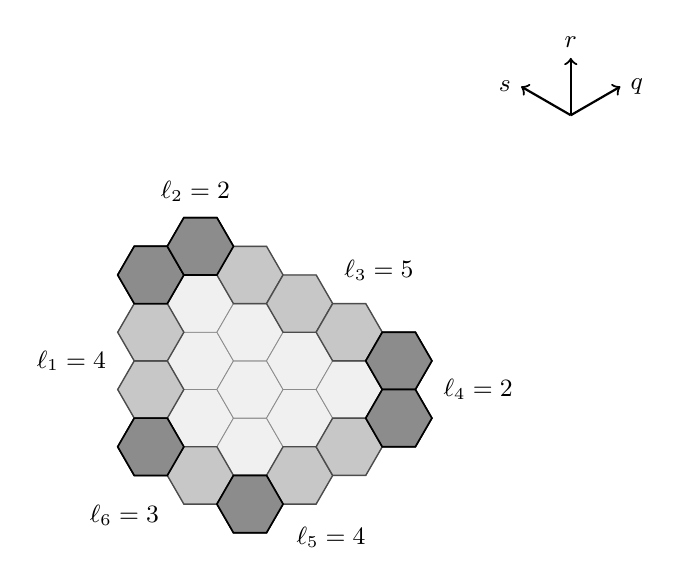
\begin{tikzpicture}[scale=0.42]
  \draw[fill=black!6,draw=black!45,line width=0.3pt] (1.000,3.464) -- (0.500,4.330) -- (-0.500,4.330) -- (-1.000,3.464) -- (-0.500,2.598) -- (0.500,2.598) -- cycle;
  \draw[fill=black!6,draw=black!45,line width=0.3pt] (1.000,5.196) -- (0.500,6.062) -- (-0.500,6.062) -- (-1.000,5.196) -- (-0.500,4.330) -- (0.500,4.330) -- cycle;
  \draw[fill=black!6,draw=black!45,line width=0.3pt] (1.000,6.928) -- (0.500,7.794) -- (-0.500,7.794) -- (-1.000,6.928) -- (-0.500,6.062) -- (0.500,6.062) -- cycle;
  \draw[fill=black!6,draw=black!45,line width=0.3pt] (1.000,8.660) -- (0.500,9.526) -- (-0.500,9.526) -- (-1.000,8.660) -- (-0.500,7.794) -- (0.500,7.794) -- cycle;
  \draw[fill=black!6,draw=black!45,line width=0.3pt] (2.500,2.598) -- (2.000,3.464) -- (1.000,3.464) -- (0.500,2.598) -- (1.000,1.732) -- (2.000,1.732) -- cycle;
  \draw[fill=black!6,draw=black!45,line width=0.3pt] (2.500,4.330) -- (2.000,5.196) -- (1.000,5.196) -- (0.500,4.330) -- (1.000,3.464) -- (2.000,3.464) -- cycle;
  \draw[fill=black!6,draw=black!45,line width=0.3pt] (2.500,6.062) -- (2.000,6.928) -- (1.000,6.928) -- (0.500,6.062) -- (1.000,5.196) -- (2.000,5.196) -- cycle;
  \draw[fill=black!6,draw=black!45,line width=0.3pt] (2.500,7.794) -- (2.000,8.660) -- (1.000,8.660) -- (0.500,7.794) -- (1.000,6.928) -- (2.000,6.928) -- cycle;
  \draw[fill=black!6,draw=black!45,line width=0.3pt] (2.500,9.526) -- (2.000,10.392) -- (1.000,10.392) -- (0.500,9.526) -- (1.000,8.660) -- (2.000,8.660) -- cycle;
  \draw[fill=black!6,draw=black!45,line width=0.3pt] (4.000,1.732) -- (3.500,2.598) -- (2.500,2.598) -- (2.000,1.732) -- (2.500,0.866) -- (3.500,0.866) -- cycle;
  \draw[fill=black!6,draw=black!45,line width=0.3pt] (4.000,3.464) -- (3.500,4.330) -- (2.500,4.330) -- (2.000,3.464) -- (2.500,2.598) -- (3.500,2.598) -- cycle;
  \draw[fill=black!6,draw=black!45,line width=0.3pt] (4.000,5.196) -- (3.500,6.062) -- (2.500,6.062) -- (2.000,5.196) -- (2.500,4.330) -- (3.500,4.330) -- cycle;
  \draw[fill=black!6,draw=black!45,line width=0.3pt] (4.000,6.928) -- (3.500,7.794) -- (2.500,7.794) -- (2.000,6.928) -- (2.500,6.062) -- (3.500,6.062) -- cycle;
  \draw[fill=black!6,draw=black!45,line width=0.3pt] (4.000,8.660) -- (3.500,9.526) -- (2.500,9.526) -- (2.000,8.660) -- (2.500,7.794) -- (3.500,7.794) -- cycle;
  \draw[fill=black!6,draw=black!45,line width=0.3pt] (5.500,2.598) -- (5.000,3.464) -- (4.000,3.464) -- (3.500,2.598) -- (4.000,1.732) -- (5.000,1.732) -- cycle;
  \draw[fill=black!6,draw=black!45,line width=0.3pt] (5.500,4.330) -- (5.000,5.196) -- (4.000,5.196) -- (3.500,4.330) -- (4.000,3.464) -- (5.000,3.464) -- cycle;
  \draw[fill=black!6,draw=black!45,line width=0.3pt] (5.500,6.062) -- (5.000,6.928) -- (4.000,6.928) -- (3.500,6.062) -- (4.000,5.196) -- (5.000,5.196) -- cycle;
  \draw[fill=black!6,draw=black!45,line width=0.3pt] (5.500,7.794) -- (5.000,8.660) -- (4.000,8.660) -- (3.500,7.794) -- (4.000,6.928) -- (5.000,6.928) -- cycle;
  \draw[fill=black!6,draw=black!45,line width=0.3pt] (7.000,3.464) -- (6.500,4.330) -- (5.500,4.330) -- (5.000,3.464) -- (5.500,2.598) -- (6.500,2.598) -- cycle;
  \draw[fill=black!6,draw=black!45,line width=0.3pt] (7.000,5.196) -- (6.500,6.062) -- (5.500,6.062) -- (5.000,5.196) -- (5.500,4.330) -- (6.500,4.330) -- cycle;
  \draw[fill=black!6,draw=black!45,line width=0.3pt] (7.000,6.928) -- (6.500,7.794) -- (5.500,7.794) -- (5.000,6.928) -- (5.500,6.062) -- (6.500,6.062) -- cycle;
  \draw[fill=black!6,draw=black!45,line width=0.3pt] (8.500,4.330) -- (8.000,5.196) -- (7.000,5.196) -- (6.500,4.330) -- (7.000,3.464) -- (8.000,3.464) -- cycle;
  \draw[fill=black!6,draw=black!45,line width=0.3pt] (8.500,6.062) -- (8.000,6.928) -- (7.000,6.928) -- (6.500,6.062) -- (7.000,5.196) -- (8.000,5.196) -- cycle;
  \draw[fill=black!22,draw=black!70,line width=0.5pt] (1.000,3.464) -- (0.500,4.330) -- (-0.500,4.330) -- (-1.000,3.464) -- (-0.500,2.598) -- (0.500,2.598) -- cycle;
  \draw[fill=black!22,draw=black!70,line width=0.5pt] (1.000,5.196) -- (0.500,6.062) -- (-0.500,6.062) -- (-1.000,5.196) -- (-0.500,4.330) -- (0.500,4.330) -- cycle;
  \draw[fill=black!22,draw=black!70,line width=0.5pt] (1.000,6.928) -- (0.500,7.794) -- (-0.500,7.794) -- (-1.000,6.928) -- (-0.500,6.062) -- (0.500,6.062) -- cycle;
  \draw[fill=black!22,draw=black!70,line width=0.5pt] (1.000,8.660) -- (0.500,9.526) -- (-0.500,9.526) -- (-1.000,8.660) -- (-0.500,7.794) -- (0.500,7.794) -- cycle;
  \draw[fill=black!22,draw=black!70,line width=0.5pt] (1.000,8.660) -- (0.500,9.526) -- (-0.500,9.526) -- (-1.000,8.660) -- (-0.500,7.794) -- (0.500,7.794) -- cycle;
  \draw[fill=black!22,draw=black!70,line width=0.5pt] (2.500,9.526) -- (2.000,10.392) -- (1.000,10.392) -- (0.500,9.526) -- (1.000,8.660) -- (2.000,8.660) -- cycle;
  \draw[fill=black!22,draw=black!70,line width=0.5pt] (2.500,9.526) -- (2.000,10.392) -- (1.000,10.392) -- (0.500,9.526) -- (1.000,8.660) -- (2.000,8.660) -- cycle;
  \draw[fill=black!22,draw=black!70,line width=0.5pt] (4.000,8.660) -- (3.500,9.526) -- (2.500,9.526) -- (2.000,8.660) -- (2.500,7.794) -- (3.500,7.794) -- cycle;
  \draw[fill=black!22,draw=black!70,line width=0.5pt] (5.500,7.794) -- (5.000,8.660) -- (4.000,8.660) -- (3.500,7.794) -- (4.000,6.928) -- (5.000,6.928) -- cycle;
  \draw[fill=black!22,draw=black!70,line width=0.5pt] (7.000,6.928) -- (6.500,7.794) -- (5.500,7.794) -- (5.000,6.928) -- (5.500,6.062) -- (6.500,6.062) -- cycle;
  \draw[fill=black!22,draw=black!70,line width=0.5pt] (8.500,6.062) -- (8.000,6.928) -- (7.000,6.928) -- (6.500,6.062) -- (7.000,5.196) -- (8.000,5.196) -- cycle;
  \draw[fill=black!22,draw=black!70,line width=0.5pt] (8.500,4.330) -- (8.000,5.196) -- (7.000,5.196) -- (6.500,4.330) -- (7.000,3.464) -- (8.000,3.464) -- cycle;
  \draw[fill=black!22,draw=black!70,line width=0.5pt] (8.500,6.062) -- (8.000,6.928) -- (7.000,6.928) -- (6.500,6.062) -- (7.000,5.196) -- (8.000,5.196) -- cycle;
  \draw[fill=black!22,draw=black!70,line width=0.5pt] (4.000,1.732) -- (3.500,2.598) -- (2.500,2.598) -- (2.000,1.732) -- (2.500,0.866) -- (3.500,0.866) -- cycle;
  \draw[fill=black!22,draw=black!70,line width=0.5pt] (5.500,2.598) -- (5.000,3.464) -- (4.000,3.464) -- (3.500,2.598) -- (4.000,1.732) -- (5.000,1.732) -- cycle;
  \draw[fill=black!22,draw=black!70,line width=0.5pt] (7.000,3.464) -- (6.500,4.330) -- (5.500,4.330) -- (5.000,3.464) -- (5.500,2.598) -- (6.500,2.598) -- cycle;
  \draw[fill=black!22,draw=black!70,line width=0.5pt] (8.500,4.330) -- (8.000,5.196) -- (7.000,5.196) -- (6.500,4.330) -- (7.000,3.464) -- (8.000,3.464) -- cycle;
  \draw[fill=black!22,draw=black!70,line width=0.5pt] (1.000,3.464) -- (0.500,4.330) -- (-0.500,4.330) -- (-1.000,3.464) -- (-0.500,2.598) -- (0.500,2.598) -- cycle;
  \draw[fill=black!22,draw=black!70,line width=0.5pt] (2.500,2.598) -- (2.000,3.464) -- (1.000,3.464) -- (0.500,2.598) -- (1.000,1.732) -- (2.000,1.732) -- cycle;
  \draw[fill=black!22,draw=black!70,line width=0.5pt] (4.000,1.732) -- (3.500,2.598) -- (2.500,2.598) -- (2.000,1.732) -- (2.500,0.866) -- (3.500,0.866) -- cycle;
  \draw[fill=black!45,draw=black,line width=0.6pt] (1.000,8.660) -- (0.500,9.526) -- (-0.500,9.526) -- (-1.000,8.660) -- (-0.500,7.794) -- (0.500,7.794) -- cycle;
  \draw[fill=black!45,draw=black,line width=0.6pt] (2.500,9.526) -- (2.000,10.392) -- (1.000,10.392) -- (0.500,9.526) -- (1.000,8.660) -- (2.000,8.660) -- cycle;
  \draw[fill=black!45,draw=black,line width=0.6pt] (8.500,6.062) -- (8.000,6.928) -- (7.000,6.928) -- (6.500,6.062) -- (7.000,5.196) -- (8.000,5.196) -- cycle;
  \draw[fill=black!45,draw=black,line width=0.6pt] (8.500,4.330) -- (8.000,5.196) -- (7.000,5.196) -- (6.500,4.330) -- (7.000,3.464) -- (8.000,3.464) -- cycle;
  \draw[fill=black!45,draw=black,line width=0.6pt] (4.000,1.732) -- (3.500,2.598) -- (2.500,2.598) -- (2.000,1.732) -- (2.500,0.866) -- (3.500,0.866) -- cycle;
  \draw[fill=black!45,draw=black,line width=0.6pt] (1.000,3.464) -- (0.500,4.330) -- (-0.500,4.330) -- (-1.000,3.464) -- (-0.500,2.598) -- (0.500,2.598) -- cycle;
  \node[font=\small] at (-2.40,6.06) {$ \ell_1=4 $};
  \node[font=\small] at (1.35,11.19) {$ \ell_2=2 $};
  \node[font=\small] at (6.90,8.79) {$ \ell_3=5 $};
  \node[font=\small] at (9.90,5.20) {$ \ell_4=2 $};
  \node[font=\small] at (5.45,0.73) {$ \ell_5=4 $};
  \node[font=\small] at (-0.80,1.40) {$ \ell_6=3 $};
  \draw[->,thick] (12.70,13.49) -- ++(1.5,0.866) node[right,font=\small] {$q$};
  \draw[->,thick] (12.70,13.49) -- ++(0,1.732) node[above,font=\small] {$r$};
  \draw[->,thick] (12.70,13.49) -- ++(-1.5,0.866) node[left,font=\small] {$s$};
\end{tikzpicture}
\caption{The tight hull \(H(7;1,1,2)\), with its six side lines shaded and the six corner
cells \(\kappa_{1},\dots,\kappa_{6}\) darker. The side lengths are
\(\ell_{1},\dots,\ell_{6}\) in the cyclic order of Section~\ref{sec:2.3}, namely
\(q_{\min}\), \(r_{\max}\), \(s_{\max}\), \(q_{\max}\), \(r_{\min}\), \(s_{\min}\). Here
\(\sum_{i}\ell_{i}=20=\lambda(H)+3\) and the three opposite differences all equal
\(\delta(H)=2\); the shortest side length is \(h=2\).}\label{fig:hull}
\end{figure}

\begin{remark}[attribution]\label{rem:fs}
An equivalent defect identity is obtained from F\"ulep and Sieben's polyiamond identity
\cite[Lemma~3.3]{FulepSieben2010} through the triangular--hexagonal duality developed in their Section~5.
In the same site-perimeter variables, \cite[Proposition~5.10]{FulepSieben2010} yields exactly the capacity
function $M(t)$ of Section~\ref{sec:capacity} when their perimeter variable is set equal to $t+3$; the value $7$
of that variable excluded there corresponds to the value $t=4$ excluded in
Remark~\ref{rem:attain}.
\end{remark}


\section{Capacity and minimum edge perimeter}\label{sec:capacity}

\subsection{Peeling and extremal capacity}\label{sec:2.6}

We first record the two operations on directionally convex polyhexes that the capacity
computation needs: removing a whole support trace, and putting it back one cell at a time.

\begin{lemma}[peeling]\label{lem:peel}
Let \(K\) be a directionally convex polyhex, let \(\Lambda\) be one of its six extreme
lines, and let \(K':=K\sm\Lambda\). If \(K'\neq\emptyset\), then
\begin{enumerate}
\item[(i)] \(K'\) is a directionally convex polyhex with \(\sigma(K')\le\sigma(K)-1\);
\item[(ii)] the cells of \(K\cap\Lambda\) can be ordered \(c_{1},\dots,c_{k}\) so that for
every \(j\) the set \(K'\cup\{c_{1},\dots,c_{j}\}\) is a directionally convex polyhex of
edge semiperimeter at most \(\sigma(K)\).
\end{enumerate}
\end{lemma}

\begin{proof}
Say \(\Lambda\) is the line \(q=q_{\min}\); the other five cases are the same after
permuting the roles of the keys and of the two senses.

(i) For each occupied value \(k\) of \(q\) let \(K_{k}\) be the trace of \(K\) on
\(q=k\); it is a run. If \(K\) is connected, then for consecutive values \(k,k+1\) a path
inside \(K\) joining a cell of \(K_{k}\) to a cell of \(K_{k+1}\) must, by
Fact~\ref{f:3}, contain a step from a cell with \(q=k\) to a cell with \(q=k+1\), so
\(K_{k}\) and \(K_{k+1}\) are adjacent. Hence \(K'\), the union of the \(K_{k}\) with
\(k\ge q_{\min}+1\), is connected. Its traces in the \(q\)-family are traces of \(K\),
hence runs. Now fix a line of the \(r\)-family, \(r=k\); its cells are \((q,k)\), so the
trace of \(K\) on it is a run if and only if its \(q\)-values form an interval, and by
Fact~\ref{f:2} it meets \(\Lambda\) in at most the one cell \((q_{\min},k)\). The trace of
\(K'\) on this line is the trace of \(K\) with that cell, if present, removed. Since
\(q_{\min}\) is the least \(q\)-value occurring anywhere in \(K\), it is the least
\(q\)-value of the interval, so removing it leaves an interval, possibly empty. A line of
the \(s\)-family, \(s=k\), has cells \((q,k-q)\), again parametrized by \(q\), and the
same sentence applies verbatim. So all traces of \(K'\) are runs and \(K'\) is
directionally convex. Finally \(\Lambda\) is occupied by
\(K\) and not by \(K'\), so \(\lambda(K')\le\lambda(K)-1\), and by Lemma~\ref{lem:runs}
\(\sigma(K')=\lambda(K')\le\lambda(K)-1=\sigma(K)-1\).

(ii) Since \(K\) is connected there is a cell \(c_{1}\in K\cap\Lambda\) adjacent to
\(K'\). Order the remaining cells of the run \(K\cap\Lambda\) so that every initial
segment \(\{c_{1},\dots,c_{j}\}\) is a block of consecutive cells of that run containing
\(c_{1}\). Write \(K_{j}:=K'\cup\{c_{1},\dots,c_{j}\}\). Then \(K_{j}\) is connected,
because \(c_{1}\) is adjacent to \(K'\) and each later \(c_{j}\) is adjacent to a cell
already inserted. Its trace on \(\Lambda\) is a block, hence a run; its trace on any other
line of the \(q\)-family is a trace of \(K'\), hence a run. On a line of the \(r\)- or
\(s\)-family, parametrized by \(q\) as in (i), the trace of \(K_{j}\) is the trace of
\(K'\) there together with at most one inserted cell, which lies on \(\Lambda\) and so
has \(q=q_{\min}\). The trace of \(K\) on that line is a run containing this cell and, by
(i), the trace of \(K'\) is that run with its least element \(q_{\min}\) removed; putting
the cell back restores the run of \(K\). Hence every trace of \(K_{j}\) is a run, so
\(K_{j}\) is directionally convex, and every line it occupies is occupied by \(K\), whence
\(\sigma(K_{j})=\lambda(K_{j})\le\lambda(K)=\sigma(K)\).
\end{proof}

\begin{corollary}\label{cor:subsets}
Let \(K\) be a directionally convex polyhex. For every \(j\) with \(1\le j\le|K|\) there is
a directionally convex polyhex \(K_{j}\subseteq K\) with \(|K_{j}|=j\) and
\(\sigma(K_{j})\le\sigma(K)\).
\end{corollary}

\begin{proof}
Strong induction on \(|K|\). For \(|K|=1\) there is nothing to prove. Let \(|K|\ge2\). Some
extreme line \(\Lambda\) does not contain all of \(K\): otherwise \(K\) would be contained
in two extreme lines belonging to different families, which by Fact~\ref{f:2} meet in a
single cell, contradicting \(|K|\ge2\). Apply Lemma~\ref{lem:peel} to that \(\Lambda\). The
sets \(K_{j}\) of part (ii) supply all sizes between \(|K'|\) and \(|K|\); the sizes below
\(|K'|\) are supplied by the inductive hypothesis applied to \(K'\), whose edge
semiperimeter is at most \(\sigma(K)\).
\end{proof}

\begin{definition}\label{def:M}
For an integer \(t\ge0\) put
\[
   M(t):=\left\lfloor\frac{t^{2}+3}{12}\right\rfloor .
\]
Thus \(M(0)=M(1)=M(2)=0\) and \(M(3)=1\). The function \(M\) is nondecreasing.
\end{definition}

\begin{theorem}\label{thm:capacity}
Let \(N\ge1\).
\begin{enumerate}
\item[(a)] Every polyhex \(S\) satisfies \(|S|\le M(\sigma(S))\): a configuration of edge
semiperimeter \(t\) cannot have more than \(M(t)\) cells.
\item[(b)] For every \(t\ge3\) there is a directionally convex polyhex \(K\) with
\(|K|=M(t)\) and \(\sigma(K)\le t\).
\item[(c)] The minimum edge perimeter of an \(N\)-cell polyhex is
\[
   p_{\min}(N)=2g(N),\qquad g(N)=\left\lceil\sqrt{12N-3}\,\right\rceil .
\]
\item[(d)] Every \(N\)-cell minimizer \(S\) is directionally convex and satisfies
\(\sigma(S)=\lambda(S)=g(N)\).
\end{enumerate}
\end{theorem}

The directional convexity of minimizers in (d) is a known result. Davoli, Piovano and
Stefanelli \cite[Definition~3.2 and Proposition~3.3]{DavoliPiovanoStefanelli2017}
establish this property for every minimizer of the edge-isoperimetric problem on the
triangular lattice. Their original preprint calls the property \emph{$3$-connected}:
for any two points on a common lattice line, all lattice points between them belong
to the set. Under the identification of Section~\ref{sec:0.5} this is exactly the
directional convexity used here. Their proof uses rearrangement; the proof below
obtains (d) from the hull identities of Section~\ref{sec:hulls} and the capacity
bound (a), together with $\lambda(S)=g(N)$, to keep the argument self-contained.

\begin{proof}
(a) Let \(H=H(S)\). By Lemma~\ref{lem:hull} and Lemma~\ref{lem:hex}(v),
\[
   12|S|\le12|H|=\lambda(H)^{2}+3-\bigl(3\delta(H)^{2}+2Q(H)\bigr)\le\lambda(S)^{2}+3
   \le\sigma(S)^{2}+3 ,
\]
the last step by Lemma~\ref{lem:runs}. Since \(|S|\) is an integer, \(|S|\le M(\sigma(S))\).

(b) For \(t\equiv3\pmod 6\), say \(t=6m+3\), take \(K=H(3m+1;m,m,m)\); for \(t=6m\) take
\(H(3m-1;m-1,m-1,m-1)\); for \(t=6m+1\) take \(H(3m;m,m,m-1)\); for \(t=6m+2\) take
\(H(3m+1;m,m,m+1)\); for \(t=6m+4\) take \(H(3m+1;m,m,m-1)\); for \(t=6m+5\) take
\(H(3m+2;m,m,m+1)\). Here \(m\ge0\) for \(t\equiv3,5\pmod6\) and \(m\ge1\)
for the other four residues, which covers every \(t\ge3\) except \(t=4\); in each case
\eqref{eq:adm} holds, Lemma~\ref{lem:hex}(ii) gives \(\sigma(K)=t\), and
Lemma~\ref{lem:hex}(iv),(v) give
\(12|K|=t^{2}+3-D\) with \(D\in\{0,3,4,7\}\) according to the residue of \(t\), so
\(|K|=M(t)\). The single case not covered by an admissible triple is \(t=4\); there
\(M(4)=1\) and a single cell has edge semiperimeter \(3\le4\).

(c) Put \(t_{N}:=\min\{t\ge3:\ M(t)\ge N\}\). By (a) every \(N\)-cell polyhex has
\(M(\sigma(S))\ge N\), hence \(\sigma(S)\ge t_{N}\). Conversely (b) produces a
directionally convex \(K\) with \(|K|=M(t_{N})\ge N\) and \(\sigma(K)\le t_{N}\), and
Corollary~\ref{cor:subsets} extracts from it an \(N\)-cell polyhex of edge semiperimeter at
most \(t_{N}\). Therefore \(p_{\min}(N)=2t_{N}\). Finally, for integers \(t\),
\[
   M(t)\ge N\iff \frac{t^{2}+3}{12}\ge N\iff t\ge\sqrt{12N-3},
\]
and \(\sqrt{12N-3}\ge3\) for \(N\ge1\), so \(t_{N}=g(N)\).

(d) By (c), \(\sigma(S)=g(N)\). Let \(H=H(S)\). Applying (a) to \(H\), which is
directionally convex with \(\sigma(H)=\lambda(H)\), gives \(M(\lambda(H))\ge|H|\ge N\) and
therefore \(\lambda(H)\ge t_{N}=g(N)\). Combining with Lemmas~\ref{lem:runs}
and~\ref{lem:hull},
\[
   g(N)=\sigma(S)=R(S)\ \ge\ \lambda(S)=\lambda(H)\ \ge\ g(N),
\]
so \(R(S)=\lambda(S)\) and \(S\) is directionally convex.
\end{proof}

\begin{remark}\label{rem:attain}
Parts (a) and (b) together say exactly that
\[
   M(t)=\max\{\,|K|:\ K\text{ a polyhex with }\sigma(K)\le t\,\},
\]
in words: \(M(t)\) is the largest number of cells that fit within an edge-semiperimeter
budget of \(t\). The budget form is the one the rest of the paper uses, and the
inequality in (b) is not a weakening: for every \(t\ge3\) other than \(t=4\) the
hexagons listed in the proof do satisfy \(\sigma(K)=t\), and the value \(t=4\) is not the
edge semiperimeter of any polyhex at all. Indeed a polyhex \(K\) with \(\sigma(K)=4\)
would have \(|K|\le M(4)=1\) by (a), while the one-cell polyhex has edge semiperimeter
\(3\).
\end{remark}

\subsection{The plateau bridge}\label{sec:2.7}

The function \(N\mapsto g(N)\) is nondecreasing and takes each of its values on a block of
consecutive integers. For \(\gamma\) in the range of \(g\) let
\[
   N_{b}(\gamma):=\min\{\,N\ge1:\ g(N)=\gamma\,\}
\]
be the first cell count at which the minimum edge semiperimeter equals \(\gamma\).

\begin{lemma}\label{lem:bridge}
For every \(\gamma\) in the range of \(g\),
\begin{equation}\label{eq:bridge}
   N_{b}(\gamma)=M(\gamma-1)+1 ,
\end{equation}
in words: the plateau on which the minimum edge semiperimeter equals \(\gamma\) begins one
cell after the capacity of edge semiperimeter \(\gamma-1\) has been exhausted.
\end{lemma}

\begin{proof}
For integers \(N\ge1\) and \(t\ge3\) we have, as in the proof of
Theorem~\ref{thm:capacity}(c), \(g(N)\le t\) if and only if \(N\le M(t)\). Hence
\(\{N:\ g(N)\le\gamma-1\}=\{1,\dots,M(\gamma-1)\}\), so the least \(N\) with
\(g(N)\ge\gamma\) is \(M(\gamma-1)+1\); as \(\gamma\) lies in the range of \(g\), that
least \(N\) satisfies \(g(N)=\gamma\).
\end{proof}

Lemma~\ref{lem:bridge} is used in Section~\ref{sec:skeleton} to recognize when a
minimizer sits at the start of its plateau.


\section{The shortest side and rigidity at exceptional plateau starts}\label{sec:rigidity}

Throughout this section \(S\) is an edge-perimeter minimizer with \(n=|S|\) and
\(\sigma=\sigma(S)=g(n)\); by Theorem~\ref{thm:capacity}(d) it is directionally convex, so
its support traces \(r_{i}\) and \(\rho(S)=\min_{i}r_{i}\) are defined, and by
Lemma~\ref{lem:hull}(iii) \(\rho(S)\ge1\). Let \(H=H(S)\).

A word on terminology, since four related phrases occur side by side from here on. The
six \emph{extreme lines} \(\Lambda_{i}\) of \(S\) (Section~\ref{sec:2.3}) are the same six
lines as the \emph{side lines} of \(H\) (Lemma~\ref{lem:hull}(ii)). On each of them there
are two sets: the \emph{side} \(H\cap\Lambda_{i}\) of the hull, of length \(\ell_{i}\), and the
\emph{support trace} \(S\cap\Lambda_{i}\) of the configuration, of length \(r_{i}\). A
\emph{shortest side} refers to \(\min_{i}\ell_{i}=h\), a \emph{shortest extreme line} or
\emph{shortest support trace} to \(\min_{i}r_{i}=\rho(S)\). The theorem of
Section~\ref{sec:skeleton} deletes a shortest support trace; the rigidity argument below
compares it with the sides.

\begin{observation}\label{obs:fullside}
Let \(S\) be a directionally convex polyhex with tight hull \(H\).
\begin{enumerate}
\item[(a)] For every \(i\), \(S\cap\Lambda_{i}\subseteq H\cap\Lambda_{i}\), so
\(r_{i}\le\ell_{i}\), and \(r_{i}=\ell_{i}\) holds if and only if
\(S\cap\Lambda_{i}=H\cap\Lambda_{i}\), that is, the whole side lies in \(S\).
\item[(b)] If the two sides adjacent to \(H\cap\Lambda_{i}\) in the cyclic order, namely
\(H\cap\Lambda_{i-1}\) and \(H\cap\Lambda_{i+1}\), are contained in \(S\), then so is
the side \(H\cap\Lambda_{i}\).
\end{enumerate}
\end{observation}

\begin{proof}
(a) is Lemma~\ref{lem:hull}(i) restricted to \(\Lambda_{i}\): two finite sets, one inside
the other, have the same cardinality exactly when they coincide. For (b), the corners
\(\kappa_{i-1}=H\cap\Lambda_{i-1}\cap\Lambda_{i}\) and \(\kappa_{i}=H\cap\Lambda_{i}\cap\Lambda_{i+1}\)
lie on the two complete sides and hence in \(S\). By Lemma~\ref{lem:hex}(i) they are the
two end cells of the run \(H\cap\Lambda_{i}\); the trace \(S\cap\Lambda_{i}\) is a run
containing both ends of that run, so it contains the whole of it.
\end{proof}

\begin{lemma}\label{lem:rhobound}
\(\displaystyle \rho(S)\le\Bigl\lfloor\frac{\sigma+3}{6}\Bigr\rfloor\). In words: the shortest
support trace has at most one sixth of \(\sigma+3\) cells.
\end{lemma}

\begin{proof}
By Lemma~\ref{lem:hull}(ii) and \eqref{eq:sidesum}, \(\sum_{i}\ell_{i}=\lambda(H)+3=\sigma+3\).
Since \(S\subseteq H\), \(r_{i}\le\ell_{i}\), so \(\sum_{i}r_{i}\le\sigma+3\); the minimum of
six integers is at most their mean.
\end{proof}

The bound is attained by hulls whose six sides are as equal as they can be, and this is
exactly what happens at the start of certain plateaux. The next proposition, the only
delicate step of the paper, says that at those plateau starts a minimizer cannot have all
six support traces that long.

\begin{proposition}[rigidity at exceptional plateau starts]\label{pro:rigidity}
Let \(m\ge1\), let \(\gamma\) be in the range of \(g\) with \(\gamma\in\{6m+3,\ 6m+5\}\),
and let \(S\) be an edge-perimeter minimizer with \(|S|=N_{b}(\gamma)\). Then
\(\rho(S)\le m\).
\end{proposition}

In words: at the start of a plateau whose threshold is \(3\) or \(5\) modulo \(6\), the
shortest support trace of a minimizer is strictly shorter than the bound of
Lemma~\ref{lem:rhobound}, which there equals \(m+1\).

\begin{proof}
Put \(N=N_{b}(\gamma)\). By Lemma~\ref{lem:bridge}, \(N=M(\gamma-1)+1\), which for the two
residues gives
\begin{equation}\label{eq:nbspecial}
   N_{b}(6h-3)=3h^{2}-4h+2,\qquad N_{b}(6h-1)=3h^{2}-2h+1\qquad(h=m+1),
\end{equation}
since \(\bigl((6h-4)^{2}+3\bigr)/12\) has integer part \(3h^{2}-4h+1\) and
\(\bigl((6h-2)^{2}+3\bigr)/12\) has integer part \(3h^{2}-2h\). By
Theorem~\ref{thm:capacity}(d), \(S\) is directionally convex with \(\lambda(S)=\gamma\),
hence \(\lambda(H)=\gamma\) by Lemma~\ref{lem:hull}(ii).

\medskip\noindent\textbf{Case \(\gamma\equiv3\pmod6\).} Write \(\gamma=6h-3\), so
\(h=m+1\ge2\). We must show \(\rho(S)\le h-1\). Suppose \(\rho(S)\ge h\). Then every
support trace has at least \(h\) cells, so every side of the hull has \(\ell_{i}\ge r_{i}\ge h\);
as \(\sum_{i}\ell_{i}=\gamma+3=6h\) by \eqref{eq:sidesum} and Lemma~\ref{lem:hull}(ii), all
six sides equal \(h\). Solving
\(\ell_{2}=v+1=\ell_{4}=u+1=\ell_{6}=w+1=h\) and \(\ell_{1}=L-v-w=h\) gives
\[
   u=v=w=h-1,\qquad L=3h-2,
\]
so by Lemma~\ref{lem:hex}(iv)
\[
   |H|=T(3h-2)-3\,T(h-1)=3h^{2}-3h+1 .
\]
By \eqref{eq:nbspecial}, \(N=3h^{2}-4h+2\), so \(|H|-N=h-1\ge1\). But \(r_{i}\ge h=\ell_{i}\)
for every \(i\) means, by Observation~\ref{obs:fullside}(a), that every side of the hull
lies entirely in \(S\), and Lemma~\ref{lem:complete} then gives \(S=H\), contradicting
\(|S|=N<|H|\).

\medskip\noindent\textbf{Case \(\gamma\equiv5\pmod6\).} Write \(\gamma=6h-1\), so again
\(h=m+1\ge2\), and suppose \(\rho(S)\ge h\). As before every side has \(\ell_{i}\ge h\), while
now \(\sum_{i}\ell_{i}=\gamma+3=6h+2\); hence the shortest side has length exactly \(h\) and
\(\sum_{i}x_{i}=2\). By Lemma~\ref{lem:oppair}
exactly one pair of opposite sides has length \(h+1\). The three families are permuted
cyclically by the \(120^{\circ}\) rotation of the lattice, which maps polyhexes to
polyhexes, preserves adjacency, perimeter and the six extreme lines as a set, and maps the
tight hull of \(S\) to the tight hull of the rotated \(S\) (the normalization of
Definition~\ref{def:hull} is re-applied after rotating); so we may assume that pair is
\((\ell_{1},\ell_{4})\), the two sides of the \(q\)-family. Solving
\(\ell_{4}=u+1=h+1\), \(\ell_{2}=v+1=h\), \(\ell_{6}=w+1=h\) and \(\ell_{1}=L-v-w=h+1\)
gives
\[
   u=h,\qquad v=w=h-1,\qquad L=3h-1
\]
(one checks \(\ell_{3}=\ell_{5}=h\) and \(\lambda(H)=3L-(u+v+w)=6h-1=\gamma\)), and
\[
   |H|=T(3h-1)-T(h)-2\,T(h-1)=3h^{2}-h .
\]
By \eqref{eq:nbspecial}, \(N=3h^{2}-2h+1\), so again \(|H|-N=h-1\ge1\).

From \(r_{i}\ge h\) and Observation~\ref{obs:fullside}(a) it follows that the four sides
of length \(h\), namely \(H\cap\Lambda_{i}\) for \(i=2,3,5,6\), are contained in \(S\).
The long side \(H\cap\Lambda_{1}\) is adjacent in the cyclic order to \(H\cap\Lambda_{6}\)
and \(H\cap\Lambda_{2}\), both contained in \(S\), so Observation~\ref{obs:fullside}(b)
puts \(H\cap\Lambda_{1}\) in \(S\) as well; the opposite side \(H\cap\Lambda_{4}\) is
handled in the same way through its neighbours \(H\cap\Lambda_{3}\) and
\(H\cap\Lambda_{5}\). So all six sides are contained in \(S\), and
Lemma~\ref{lem:complete} gives \(S=H\), contradicting \(|S|=N<|H|\).
\end{proof}

The logical role of Proposition~\ref{pro:rigidity} in the next section is a single
integer. Counting alone (Lemma~\ref{lem:rhobound} together with \(n\ge M(\sigma-1)+1\))
gives, after deleting a shortest support trace of length \(\rho\), the bound
\(n-\rho\ge M(\sigma-2)+1\) in four residue classes of \(\sigma\) modulo \(6\), but only
the weaker \(n-\rho\ge M(\sigma-2)\) when \(\sigma\equiv3,5\pmod6\), with equality
exactly at a plateau start with \(\rho=m+1\). The proposition rules out that equality
case, and thereby raises the weak bound to the strict integer bound
\(n-\rho\ge M(\sigma-2)+1\) in those two classes as well. That one unit is what makes
the peeled configuration a minimizer in Step~4 of the proof of Theorem~\ref{thm:skel}.


\section{The shortest-side skeleton theorem}\label{sec:skeleton}

\begin{theorem}[shortest-side skeleton; Theorem~\ref{thm:intro-skel}]\label{thm:skel}
Let \(S\) be an edge-perimeter minimizer with \(n=|S|\ge3\), let \(\sigma=\sigma(S)=g(n)\),
and let \(\Lambda\) be \emph{any} extreme line of \(S\) with \(|S\cap\Lambda|=\rho(S)\). Put
\(S':=S\sm\Lambda\). Then
\begin{enumerate}
\item[(i)] \(S'\) is nonempty and is an edge-perimeter minimizer with \(g(|S'|)=\sigma-1\);
\item[(ii)] the cells of \(S\cap\Lambda\) can be ordered \(c_{1},\dots,c_{\rho}\) so that each
\(T_{j}:=S'\cup\{c_{1},\dots,c_{j}\}\) is a directionally convex polyhex with
\(\exc(T_{j})\le2\).
\end{enumerate}
\end{theorem}

In words: peeling a shortest extreme line from a minimizer lands on a minimizer one
threshold step down, and putting the line back one cell at a time never costs more than two
units of edge perimeter.

\begin{proof}
By Theorem~\ref{thm:capacity}(d), \(S\) is directionally convex with \(\lambda(S)=\sigma\),
and \(\rho=\rho(S)\ge1\). Since \(n\ge3\), \(g(3)=\lceil\sqrt{33}\rceil=6\), and \(g\) is
nondecreasing, we have \(\sigma\ge6\). Write \(\sigma=6m+s\) with \(0\le s\le5\); then
\(m\ge1\).

\medskip\noindent\textbf{Step 1 (the two bounds).}
Lemma~\ref{lem:rhobound} gives \(\rho\le\lfloor(\sigma+3)/6\rfloor\), and \(g(n)=\sigma\)
means \(n>M(\sigma-1)\), that is
\begin{equation}\label{eq:nbound}
   n\ \ge\ M(\sigma-1)+1 .
\end{equation}

\medskip\noindent\textbf{Step 2 (the residue table).}
For \(t=6m+j\) with \(0\le j\le5\), \(M(t)=3m^{2}+mj+\lfloor(j^{2}+3)/12\rfloor\), and
\(\lfloor(j^{2}+3)/12\rfloor=0,0,0,1,1,2\) for \(j=0,\dots,5\). Taking differences
(for \(s=0\) both arguments \(\sigma-1,\sigma-2\), and for \(s=1\) the argument
\(\sigma-2\), fall into the previous block \(6(m-1)+j\)), and using
\(\lfloor(\sigma+3)/6\rfloor=m+\lfloor(s+3)/6\rfloor\):

\begin{center}
\begin{tabular}{crrr}
\hline
\(s=\sigma\bmod 6\) & \(M(\sigma-1)-M(\sigma-2)\) & \(\lfloor(\sigma+3)/6\rfloor\) & difference \\
\hline
0 & \(m\)   & \(m\)   & \(0\) \\
1 & \(m\)   & \(m\)   & \(0\) \\
2 & \(m\)   & \(m\)   & \(0\) \\
3 & \(m\)   & \(m+1\) & \(-1\) \\
4 & \(m+1\) & \(m+1\) & \(0\) \\
5 & \(m\)   & \(m+1\) & \(-1\) \\
\hline
\end{tabular}
\end{center}

Combining the two bounds of Step 1,
\(n-\rho\ge M(\sigma-1)+1-\lfloor(\sigma+3)/6\rfloor\). If \(s\notin\{3,5\}\) the table
gives \(M(\sigma-1)-\lfloor(\sigma+3)/6\rfloor\ge M(\sigma-2)\), hence
\begin{equation}\label{eq:strict}
   n-\rho\ \ge\ M(\sigma-2)+1 .
\end{equation}
If \(s\in\{3,5\}\) the table gives only \(n-\rho\ge M(\sigma-2)\), with equality if and only
if \eqref{eq:nbound} and Lemma~\ref{lem:rhobound} are both equalities:
\(n=M(\sigma-1)+1\) and \(\rho=m+1\). In words: the strict inequality \eqref{eq:strict}
already holds except possibly when all three of the following occur at once --- the
threshold is \(3\) or \(5\) modulo \(6\), the configuration is at the very start of its
plateau, and the shortest trace is as long as the counting allows.

\medskip\noindent\textbf{Step 3 (the exceptional case is excluded by rigidity).}
Suppose \(s\in\{3,5\}\), \(n=M(\sigma-1)+1\) and \(\rho=m+1\). By
Lemma~\ref{lem:bridge}, \(n=N_{b}(\sigma)\); also \(\sigma=g(n)\) lies in the range of \(g\)
and \(m\ge1\). So Proposition~\ref{pro:rigidity} applies with \(\gamma=\sigma\) and gives
\(\rho\le m\),
contradicting \(\rho=m+1\). Hence \eqref{eq:strict} holds in every residue.

\medskip\noindent\textbf{Step 4 (conclusion (i)).}
From \eqref{eq:strict} and the definition of \(g\), \(g(n-\rho)\ge\sigma-1\). As
\(n-\rho\ge M(\sigma-2)+1\ge1\), the set \(S'\) is nonempty, so Lemma~\ref{lem:peel}(i)
applies: \(S'\) is a directionally convex polyhex with \(\sigma(S')\le\sigma-1\). By
Lemma~\ref{lem:runs} and Theorem~\ref{thm:capacity}(c),
\[
   2(\sigma-1)\ \le\ 2g(|S'|)\ =\ p_{\min}(|S'|)\ \le\ p(S')\ =\ 2\sigma(S')\ \le\ 2(\sigma-1),
\]
so all are equalities: \(S'\) is a minimizer and \(g(|S'|)=\sigma-1\). Nothing so far
depended on which shortest line \(\Lambda\) was chosen.

\medskip\noindent\textbf{Step 5 (conclusion (ii)).}
By Lemma~\ref{lem:peel}(ii) there is an ordering \(c_{1},\dots,c_{\rho}\) of
\(S\cap\Lambda\) such that every \(T_{j}\) is a directionally convex polyhex with
\(\sigma(T_{j})\le\sigma\). As \(|T_{j}|\ge|S'|\) and \(g\) is nondecreasing,
\(g(|T_{j}|)\ge\sigma-1\). Therefore
\[
   \exc(T_{j})=p(T_{j})-2g(|T_{j}|)=2\bigl(\sigma(T_{j})-g(|T_{j}|)\bigr)
   \le2\bigl(\sigma-(\sigma-1)\bigr)=2 .
\]
In words: during the restoration the perimeter never exceeds the starting value while the
threshold is already one step lower, so the excess is at most two.
\end{proof}

\begin{corollary}[skeleton chain]\label{cor:skel}
Every edge-perimeter minimizer \(S\) admits a chain
\(S=T_{0}\supset T_{1}\supset\cdots\supset T_{k}\) of edge-perimeter minimizers with
\(|T_{k}|\le2\), each obtained from the previous one by deleting a shortest extreme line, and
\(g(|T_{i+1}|)=g(|T_{i}|)-1\) for every step.
\end{corollary}

\begin{proof}
Apply Theorem~\ref{thm:skel}(i) while \(|T_{i}|\ge3\); sizes strictly decrease.
\end{proof}

\begin{proof}[Proof of Theorem~\ref{thm:intro-main}]
Take the chain of Corollary~\ref{cor:skel}. If \(|T_{k}|=2\), then \(T_{k}\) is a domino,
which has \(\exc=0\), and either of its cells is a single cell with \(\exc=0\); extend the
chain by one step. Between consecutive members insert the configurations
\(T_{j}\) of Theorem~\ref{thm:skel}(ii), each a polyhex of excess at most \(2\). Reading the
resulting sequence from the single cell up to \(S\) gives (b). For (a), each
\(S_{k+1}=S_{k}\cup\{c\}\) is connected and \(S_{k}\) is nonempty, so \(c\) has a neighbour
in \(S_{k}\); otherwise \(\{c\}\) would be a connected component of \(S_{k+1}\) on its own.
\end{proof}

\begin{remark}[the procedure]\label{rem:algorithm}
The construction is short to state: repeatedly delete a shortest extreme line, and read the
resulting sequence of minimizers backwards, restoring each deleted line one cell at a time
from a cell adjacent to what remains. The minimizers themselves form the skeleton of the
growth; the excess \(2\) is spent only inside the restoration of a single line.
\end{remark}


\section{Optimality of the constant two}\label{sec:sharp}

Corollary~\ref{cor:skel} says that the skeleton of the growth --- the configurations at
which a whole extreme line has just been restored --- can always be taken to consist of
minimizers. This section shows that the same cannot be asked of the intermediate one-cell
stages: the constant \(2\) of Theorem~\ref{thm:intro-main} cannot be lowered. The argument
is self-contained and uses no computation: a single identity for the effect of deleting one
cell, applied to one explicit \(13\)-cell minimizer.

\subsection{The deletion identity}\label{sec:8.1}

For a finite set of cells \(S\) and \(c\in S\) write \(\dg_{S}(c)\) for the number of cells
of \(S\) adjacent to \(c\).

\begin{lemma}\label{lem:deldeg}
For every finite set of cells \(S\) and every \(c\in S\),
\begin{equation}\label{eq:deldeg}
   p(S\sm\{c\})=p(S)-6+2\dg_{S}(c) .
\end{equation}
In words: removing one cell takes away the six edges of that cell from the boundary, and
gives back, for each neighbour the cell had inside \(S\), the two sides of the shared edge
that now lie on the boundary.
\end{lemma}

\begin{proof}
Write \(n=|S|\) and \(a=a(S)\). Deleting \(c\) removes one cell and exactly
\(\dg_{S}(c)\) adjacent pairs, so \(|S\sm\{c\}|=n-1\) and
\(a(S\sm\{c\})=a-\dg_{S}(c)\). By the definition \(p(K)=6|K|-2a(K)\),
\[
   p(S\sm\{c\})=6(n-1)-2\bigl(a-\dg_{S}(c)\bigr)=\bigl(6n-2a\bigr)-6+2\dg_{S}(c),
\]
which is \eqref{eq:deldeg}.
\end{proof}

No connectedness is assumed in Lemma~\ref{lem:deldeg}; \eqref{eq:deldeg} is an identity for
arbitrary finite sets of cells. Connectedness enters only when \(S\sm\{c\}\) is to be used
as the predecessor of \(S\) in a growth chain, since a chain consists of polyhexes.

\subsection{An explicit \texorpdfstring{\(13\)}{13}-cell minimizer}\label{sec:8.2}

\begin{example}\label{ex:13}
Let
\[
   S^{\ast}:=\{(0,r):1\le r\le4\}\ \cup\ \{(1,r):0\le r\le4\}\ \cup\ \{(2,r):0\le r\le3\} .
\]
In words: three consecutive \(q\)-lines carrying \(4\), \(5\) and \(4\) cells respectively,
each a run, arranged so that the whole set is a polyhex.
\end{example}

\begin{lemma}\label{lem:13min}
The set \(S^{\ast}\) is a directionally convex polyhex with
\[
   |S^{\ast}|=13,\qquad p(S^{\ast})=26=p_{\min}(13),
\]
so \(S^{\ast}\) is a \(13\)-cell minimizer. Its degree distribution is
\[
   3^{6}\,4^{4}\,6^{3},
\]
in words: six cells of degree \(3\), four of degree \(4\) and three of degree \(6\); in
particular \(S^{\ast}\) has no cell of degree \(2\) or less.
\end{lemma}

\begin{proof}
The three traces in the \(q\)-family are the runs \(r\in[1,4]\), \(r\in[0,4]\) and
\(r\in[0,3]\), giving \(|S^{\ast}|=4+5+4=13\). The traces in the \(r\)-family are
\[
   r=0:\ q\in[1,2],\quad r=1,2,3:\ q\in[0,2],\quad r=4:\ q\in[0,1],
\]
and those in the \(s\)-family, ordered by \(q\), are
\[
   s=1:\ q\in[0,1],\quad s=2,3,4:\ q\in[0,2],\quad s=5:\ q\in[1,2].
\]
Every trace is a single run, so \(S^{\ast}\) is directionally convex, and it is connected
because consecutive \(q\)-traces overlap in their \(r\)-ranges. Counting the occupied lines
gives \(\lambda(S^{\ast})=3+5+5=13\), so by Lemma~\ref{lem:runs}
\(p(S^{\ast})=2\lambda(S^{\ast})=26\). Since \(12\cdot13-3=153\) and
\(12^{2}<153\le13^{2}\), we have \(g(13)=13\) and \(p_{\min}(13)=26\).

For the degrees, the three cells \((1,1),(1,2),(1,3)\) have all six neighbours in
\(S^{\ast}\); the four cells \((0,2),(0,3),(2,1),(2,2)\) have exactly four; and the six
cells \((0,1),(0,4),(1,0),(1,4),(2,0),(2,3)\) have exactly three. These thirteen cells
exhaust \(S^{\ast}\), and \(6\cdot3+4\cdot4+3\cdot6=52=2a(S^{\ast})\), consistent with
\(p(S^{\ast})=6\cdot13-52=26\).
\end{proof}

\subsection{No \texorpdfstring{\(12\)}{12}-cell minimizer predecessor}\label{sec:8.3}

\begin{proposition}\label{pro:nopred}
For every \(c\in S^{\ast}\),
\[
   p(S^{\ast}\sm\{c\})\ \ge\ 26\ =\ p_{\min}(12)+2 .
\]
In particular no one-cell deletion from \(S^{\ast}\) is a \(12\)-cell minimizer.
\end{proposition}

\begin{proof}
Since \(12\cdot12-3=141\) and \(11^{2}<141\le12^{2}\), we have \(g(12)=12\) and
\(p_{\min}(12)=24\). By Lemma~\ref{lem:deldeg} and \(p(S^{\ast})=26\),
\[
   p(S^{\ast}\sm\{c\})=26-6+2\dg_{S^{\ast}}(c)=20+2\dg_{S^{\ast}}(c),
\]
in words: the perimeter after the deletion is twenty plus twice the degree of the deleted
cell. Equality \(p(S^{\ast}\sm\{c\})=24\) would force \(\dg_{S^{\ast}}(c)=2\), and by
Lemma~\ref{lem:13min} no cell of \(S^{\ast}\) has degree \(2\). Every degree is at least
\(3\), so \(p(S^{\ast}\sm\{c\})\ge26\) for every \(c\).
\end{proof}

Note that connectedness of \(S^{\ast}\sm\{c\}\) never had to be examined: if the deletion
disconnects \(S^{\ast}\), the result is not a polyhex and cannot be a predecessor in a
growth chain; if it does not, Proposition~\ref{pro:nopred} already rules it out as a
minimizer. Thirteen separate case checks are not needed.

\subsection{The constant \texorpdfstring{\(2\)}{2} is optimal}\label{sec:8.4}

\begin{proof}[Proof of Theorem~\ref{thm:intro-sharp}]
Suppose there were a chain of polyhexes \(S_{1}\subset\cdots\subset S_{13}=S^{*}\) with
\(|S_{k}|=k\) and \(\exc(S_{k})=0\) for every \(k\). Then \(S_{12}\) is a polyhex with twelve cells obtained from
\(S^{\ast}\) by deleting a single cell, and \(\exc(S_{12})=0\) means
\(p(S_{12})=p_{\min}(12)=24\). This contradicts Proposition~\ref{pro:nopred}.

It remains to see that no uniform bound strictly between \(0\) and \(2\) is available. By
Lemma~\ref{lem:runs} the edge perimeter of any finite set of cells is even, and
\(p_{\min}\) is even by Theorem~\ref{thm:capacity}(c); hence
\[
   \exc(K)=p(K)-p_{\min}(|K|)\in\{0,2,4,\dots\}
\]
for every polyhex \(K\), in words: the excess is always a nonnegative even integer. A
uniform bound of \(1\) is therefore the same requirement as a uniform bound of \(0\), which
has just been refuted. So \(2\) is the least admissible constant.
\end{proof}

\begin{remark}[a second proof of Proposition~\ref{pro:nopred}]\label{rem:linecount}
Proposition~\ref{pro:nopred} also follows from line counting, which explains the example
from a different side. As computed in the proof of Lemma~\ref{lem:13min}, every one of the
thirteen lines occupied by \(S^{\ast}\) carries at least two cells: the shortest traces are
\(r=0\), \(r=4\), \(s=1\) and \(s=5\), each with exactly two. Deleting a single cell
therefore leaves every occupied line still occupied, so
\(\lambda(S^{\ast}\sm\{c\})=\lambda(S^{\ast})=13\), and Lemma~\ref{lem:runs} gives
\[
   p(S^{\ast}\sm\{c\})\ \ge\ 2\lambda(S^{\ast}\sm\{c\})\ =\ 26 .
\]
In words: no single deletion can vacate a line, so the perimeter cannot drop below twice
the unchanged line count. The degree argument of Section~\ref{sec:8.3} is shorter and is
the one we take as canonical; this one shows that the obstruction can be read off from the
support structure rather than from local degrees.
\end{remark}

Computational enumeration shows that \(N=13\) is the smallest size at which this
obstruction occurs; see Section~\ref{sec:computation}.



\section{Remarks}\label{sec:remarks}

\begin{remark}[excess alone is not a usable state space]\label{rem:x31}
Theorem~\ref{thm:intro-skel} runs its induction entirely inside the class of minimizers,
deleting a whole extreme line at a time. One might ask whether a simpler induction, deleting
one cell at a time inside the class \(\{\exc\le2\}\), could work instead. It cannot. Let
\(H\) be the regular hexagon \(H(10;3,3,3)\), which has \(37\) cells and \(\sigma(H)=21\),
and let \(X_{31}\) be \(H\) with its six corner cells removed. Each corner cell is an
end cell of the trace of \(H\) on each of the three lines through it (it is a vertex of
the convex region whose cells make up \(H\)), so removing the corners shortens traces
only at their ends. Thus \(X_{31}\) is a directionally convex polyhex with \(|X_{31}|=31\), \(\sigma(X_{31})=21\), \(g(31)=20\) and
\(\exc(X_{31})=2\); yet every line meeting \(X_{31}\) carries at least two of its cells, so
deleting any single cell leaves all \(21\) lines occupied and, since \(g(30)=19\), an excess
of at least \(2(21-19)=4\). Within \(\{\exc\le2\}\) there is no one-cell move down from
\(X_{31}\). The skeleton theorem avoids this by never leaving the minimizers except during
the restoration of a single line, where the excess is controlled by
Theorem~\ref{thm:skel}(ii) rather than by a local search.
\end{remark}

\begin{remark}[a wider class]\label{rem:nearext}
The peeling argument of Section~\ref{sec:skeleton} can be run on a larger class than the
minimizers, namely the directionally convex polyhexes \(S\) with \(|S|\ge M(\sigma(S)-1)\),
and yields one-cell growth with excess at most two for all of them. The wider class is also
closed under shortest-line peeling, but proving that closure requires a stronger
quantitative peeling estimate, obtained from a finite case analysis of the hull, rather
than the plateau-start rigidity of Proposition~\ref{pro:rigidity}; the proof is
correspondingly longer. Since the
main theorem does not need the wider class, that argument is recorded in a separate note.
\end{remark}

\begin{remark}[a one-cell-at-a-time proof]\label{rem:onecell}
Theorem~\ref{thm:intro-main} also admits a proof that descends one cell at a time, keeping
the configuration directionally convex with at most one occupied line above the threshold
and tracking two competing budgets, the length of the shortest extreme line and the
distance to the next drop of the threshold. That proof uses the same rigidity at
exceptional plateau starts as Proposition~\ref{pro:rigidity}, and in addition a local
lemma showing that a degree-two articulation cell forces excess at least four. It is
recorded separately as well.
\end{remark}



\section{Computational verification}\label{sec:computation}

No theorem of this paper depends on finite enumeration. Computation is used here for two
purposes only: to determine one size that the analytic arguments do not determine
(Section~\ref{sec:16.1}), and to re-check the statements of the paper with code written
independently of their proofs (Section~\ref{sec:16.2}).

Two different senses of ``independent'' should be kept apart. The \emph{implementations}
are independent of the proofs: the hull identities are re-derived symbolically and by
enumeration, the peeling lemma is re-checked cell by cell, and so on, without following
the steps of the argument. The \emph{enumerations of minimizers}, on the other hand, are
not logically independent of the analysis: they generate the candidates through
Theorem~\ref{thm:capacity}(d) (a minimizer is directionally convex with
\(\lambda=g(N)\)) and Section~\ref{sec:16.4} says exactly how. A row that checks a
statement on ``all minimizers with \(N\le34\)'' is therefore a check conditional on that
theorem, and two implementations of such a check are two implementations, not two
proofs. Checks that run over all polyhexes up to a given size carry no such condition.

Each entry below carries one of three labels.

\begin{center}
\begin{tabularx}{\linewidth}{@{}l>{\raggedright\arraybackslash}X@{}}
\toprule
\textsc{analytic} & The statement is proved analytically in the body; the computation is a
re-check and the proof does not rest on it. \\
\textsc{exact} & The computation enumerates a finite set completely, so it is conclusive
\emph{for that finite set}. No general theorem is made to depend on it. \\
\textsc{check} & A consistency check up to a finite size, or a census. It is not evidence
for any general statement. \\
\bottomrule
\end{tabularx}
\end{center}

\subsection{A size the proofs do not determine}\label{sec:16.1}

Section~\ref{sec:sharp} exhibits one \(13\)-cell minimizer with no all-minimizer growth chain
and proves analytically that the constant \(2\) cannot be lowered. It says nothing about
whether smaller sizes behave the same way. That is settled by enumeration.

For each \(N\le13\) we enumerated \(\mathcal{M}_{N}\) up to translation and counted the
configurations reachable from a single cell by a growth all of whose intermediate stages are
minimizers.

\begin{center}
\begin{tabular}{rrrr@{\qquad}rrrr}
\toprule
\(N\) & \(|\mathcal{M}_{N}|\) & reachable & unreachable &
\(N\) & \(|\mathcal{M}_{N}|\) & reachable & unreachable \\
\midrule
1 & 1 & 1 & 0 &  8 & 6 & 6 & 0 \\
2 & 3 & 3 & 0 &  9 & 27 & 27 & 0 \\
3 & 2 & 2 & 0 & 10 & 3 & 3 & 0 \\
4 & 3 & 3 & 0 & 11 & 24 & 24 & 0 \\
5 & 6 & 6 & 0 & 12 & 2 & 2 & 0 \\
6 & 14 & 14 & 0 & 13 & 27 & 18 & \textbf{9} \\
7 & 1 & 1 & 0 &    &    &    &   \\
\bottomrule
\end{tabular}
\end{center}

So \(N=13\) is the smallest size at which an unreachable minimizer occurs, and the
configuration \(S^{*}\) of Section~\ref{sec:sharp} is one of the nine. The \(27\)
configurations of size \(13\) form \(4\) equivalence classes under the point group of the
lattice, and the \(18\) reachable ones form \(2\) such classes. The enumeration is complete
for every \(N\le13\), so the statement that \(13\) is the smallest such size is settled
outright for that finite range. That minimality statement is a computational fact and is
not part of Theorem~\ref{thm:intro-sharp}, which needs one \(13\)-cell example and is
proved analytically. \textsc{exact}

At \(N=34\), of the \(392\) translation-normalized minimizers (\(39\) free equivalence
classes), \(102\) (\(9\) free classes) are reachable by an all-minimizer growth.
\textsc{check}

\subsection{Consistency checks}\label{sec:16.2}

Each row was carried out with an implementation written independently of the proof it
re-checks. Row 7 and the census of Section~\ref{sec:16.1} generate their minimizers
through Theorem~\ref{thm:capacity}(d) and are conditional on it in the sense explained at
the start of this section; every other row enumerates all polyhexes, all directionally
convex polyhexes or all admissible hexagons in its range, or examines a named
configuration exhaustively, and carries no such condition. No violation was found in any
of them.

\begin{center}
\footnotesize
\begin{tabularx}{\linewidth}{@{}l>{\raggedright\arraybackslash}X>{\raggedright\arraybackslash}Xl@{}}
\toprule
 & what is checked & range & status \\
\midrule
1 & \(p=2R\ge2\lambda\), and equality exactly for directionally convex sets &
all polyhexes with \(N\le11\) & \textsc{analytic} \\
2 & the hull description and the defect identity of Section~\ref{sec:hulls} &
symbolically in \(L,u,v,w\); all \(5{,}220\) admissible hexagons with \(L\le16\) &
\textsc{analytic} \\
3 & \(|S|\le M(\sigma(S))\); minimizers are directionally convex with \(\lambda=g\) &
all polyhexes with \(N\le11\) & \textsc{analytic} \\
4 & \(p_{\min}(N)=2\lceil\sqrt{12N-3}\rceil\) &
brute force for \(N\le9\); against the capacity function for \(N\le3000\) &
\textsc{analytic} \\
5 & peeling: connectedness, directional convexity and the drop in \(\sigma\) &
all \(145{,}374\) side peelings of directionally convex polyhexes with \(N\le10\) &
\textsc{analytic} \\
6 & the residue table of Section~\ref{sec:skeleton} and the two plateau-start counts
\eqref{eq:nbspecial} & \(\sigma\le2999\); \(m\le59\) & \textsc{analytic} \\
7 & Theorem~\ref{thm:skel}: every shortest-line deletion from a minimizer lands on a
minimizer with \(g\) down by one, and the restoration order keeps \(\exc\le2\) &
all \(2{,}382\) shortest-line deletions from minimizers with \(3\le N\le34\), ties included;
two independently written implementations, both enumerating minimizers via
Theorem~\ref{thm:capacity}(d) & \textsc{analytic} \\
8 & the degree table of \(S^{*}\) and its thirteen one-cell deletions &
exhaustive for \(S^{*}\) & \textsc{exact} \\
9 & the configuration \(X_{31}\) of Remark~\ref{rem:x31} & exhaustive & \textsc{exact} \\
\bottomrule
\end{tabularx}
\end{center}

For orientation: among the \(6{,}498\) deletions of a \emph{non}-shortest extreme line
from the same minimizers, only \(3{,}192\) land on a minimizer. The word ``shortest'' in
Theorem~\ref{thm:skel} is not decorative.

\subsection{Reproduction}\label{sec:16.4}

The enumeration of \(\mathcal{M}_{N}\) uses Theorem~\ref{thm:capacity}(d): a minimizer is
directionally convex with \(\lambda=g(N)\), so it suffices to enumerate the tight hulls with
the corresponding edge semiperimeter and then the subsets that keep it. For \(N\le34\) one
has \(|H|-N\le3\). Reachability is then decided by dynamic programming on the size. The
census of Section~\ref{sec:16.1} is thus exact for the class of configurations that
Theorem~\ref{thm:capacity}(d) describes; it does not re-establish that theorem.

The scripts reproducing every number quoted above are provided as ancillary files; they use
the Python standard library only and need no input files.



\section*{Statement on the use of AI-assisted tools}

AI-assisted tools (Claude and ChatGPT) were used during proof search, counterexample search,
computational verification, auditing, and preparation of the manuscript. The author evaluated
the resulting arguments and computations and is responsible for the mathematical content of the
paper.

\bibliographystyle{plain}
\bibliography{refs}

\end{document}
